\documentclass[11pt, a4paper]{article}
\usepackage[latin1]{inputenc}
\usepackage{pgfplots}
\usepackage{pgfplotstable}
\usepackage{float}
\pgfplotsset{width=0.85\textwidth ,compat=1.9}
\usepackage[dutch]{babel}
\usepackage{csquotes}
\usepackage{amsmath}
\usepackage[toc,page]{appendix}
\usepackage{amsfonts}
\usepackage{amssymb}
\usepackage{graphicx}
\usepackage{caption}
%\usepackage[backend=biber, style=numeric, citestyle=numeric-comp, sorting = none]{biblatex}
\usepackage[backend=bibtex, style=numeric, citestyle=numeric-comp]{biblatex}
\author{Stef Tweepenninckx, r0677232}
\title{Practicum 3: Image Compositing algoritme}



%define printtitle
\makeatletter
\def\printtitle{                 
    {\large \@title}} 
\makeatother

%define printauthor
\makeatletter                       
\def\printauthor{                  
    {\large \@author}}              
\makeatother

\begin{document}
\begin{titlepage}
\newcommand{\HRule}{\rule{\linewidth}{0.5mm}} 
\center 
\textsc{\LARGE Gegevensstructuren en algoritmen}\\[1.5cm] 
\HRule \\[0.4cm]

{\huge \bfseries \printtitle}\\[0.4cm] 
\HRule \\[0.4cm]

\Large \emph{Author:}\\
 \textsc{\printauthor}\\[3cm]

{\large \textsc{18 mei 2018}}\\[3cm] 

\vfill 
\end{titlepage}

\section*{Inleiding}

\section*{Kortste pad}
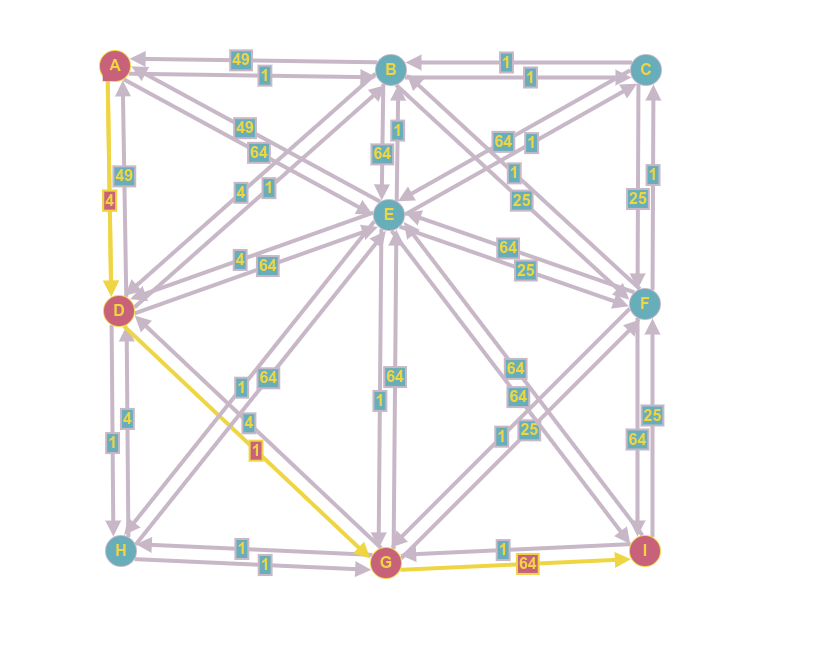
\includegraphics[width=\textwidth]{grafe}
\captionof{figure}{Grafe met aangeduid kortste pad}
\vspace*{10px}
Het resulterende kortste pad, aangeduid in het geel, is: $$A \implies D \implies G \implies I$$ met een totale kost van $49 + 4 + 1 + 64 = 118$.

\section*{Andere afstandsfunctie}
\section*{Tijdscomplexiteit}
\section*{Voorkomen van complexe vormen seam}
\section*{Langste pad ipv kortste pad}


\newpage
\end{document}
